\documentclass[a4paper]{article}
\usepackage{amsthm}
\usepackage{amsmath} % Define various maths environments
\usepackage{amssymb} % Define various maths symbols
\usepackage{mathrsfs}
\usepackage{geometry} % Adjust the margin, paper size, and etc.
\usepackage{enumerate} % Provide different style of lists
\usepackage{graphicx}
\usepackage{float}
\usepackage{multirow}
\geometry{a4paper,scale=0.78}

\title{—————————————————————————\\ \sc{UM-SJTU Joint Institute}}
\author{\sc{Computer Networks}}
\date{\sc{(Ve489)}\\——————————————————————————————}

\begin{document}
\maketitle
\vspace{5cm}
\centerline{\Large{\sc{Term Project Report}}}
\vspace{9cm}
\begin{tabular}{lll}
\qquad \qquad Name: Sun Yiwen&ID: 517370910213\\
\qquad \qquad Date: August 1 2020
\end{tabular}

\newpage
\section{Mininet and Socket Programming}
\subsection{Simple Experiments}
\begin{enumerate}
\item
\textbf{Link latency using ping.}
\par
The average round-trip time (RTT) between ($h_1$ and $h_2$) is $$\dfrac{41.9+42.4+40.8+41.5+41.7+40.6+41.1+41.8+42.4+41.5}{10}=41.57ms.$$ Link $L_1$ is used and the link latency of $L_1$ is $20ms$. The round-trip time is close to 2 times link latency.
\begin{figure}[htbp]
\centering
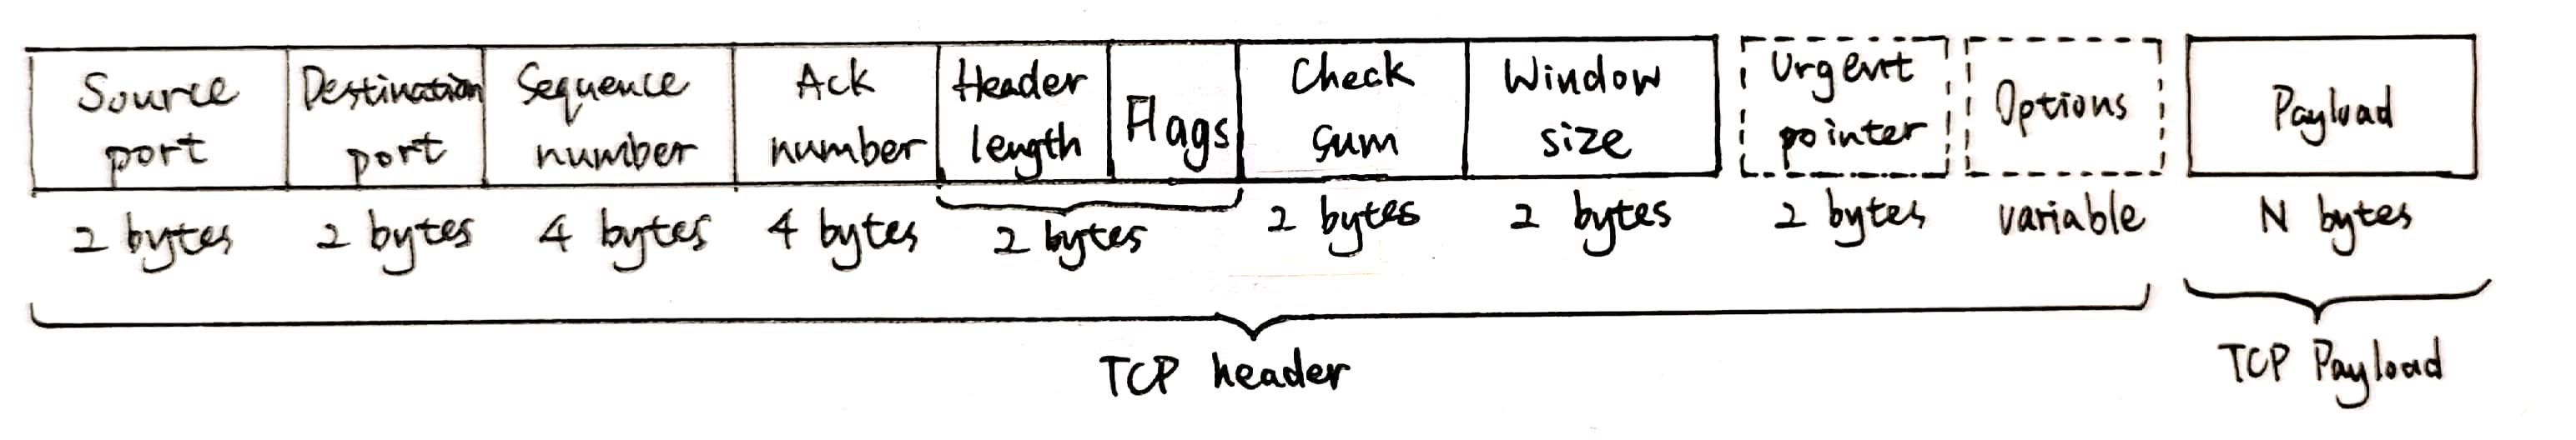
\includegraphics[scale=1]{1.jpg}
\caption{Screenshot of pinging 10 times from $h_1$ to $h_2$.}
\end{figure}
\par
The average round-trip time (RTT) between ($h_3$ and $h_5$) is $$\dfrac{21.9+21.1+21.0+21.3+21.2+20.5+21.6+21.6+21.3+21.3}{10}=21.28ms.$$ Link $L_4$ is used and the link latency of $L_4$ is $10ms$. The round-trip time is close to 2 times link latency.
\begin{figure}[htbp]
\centering
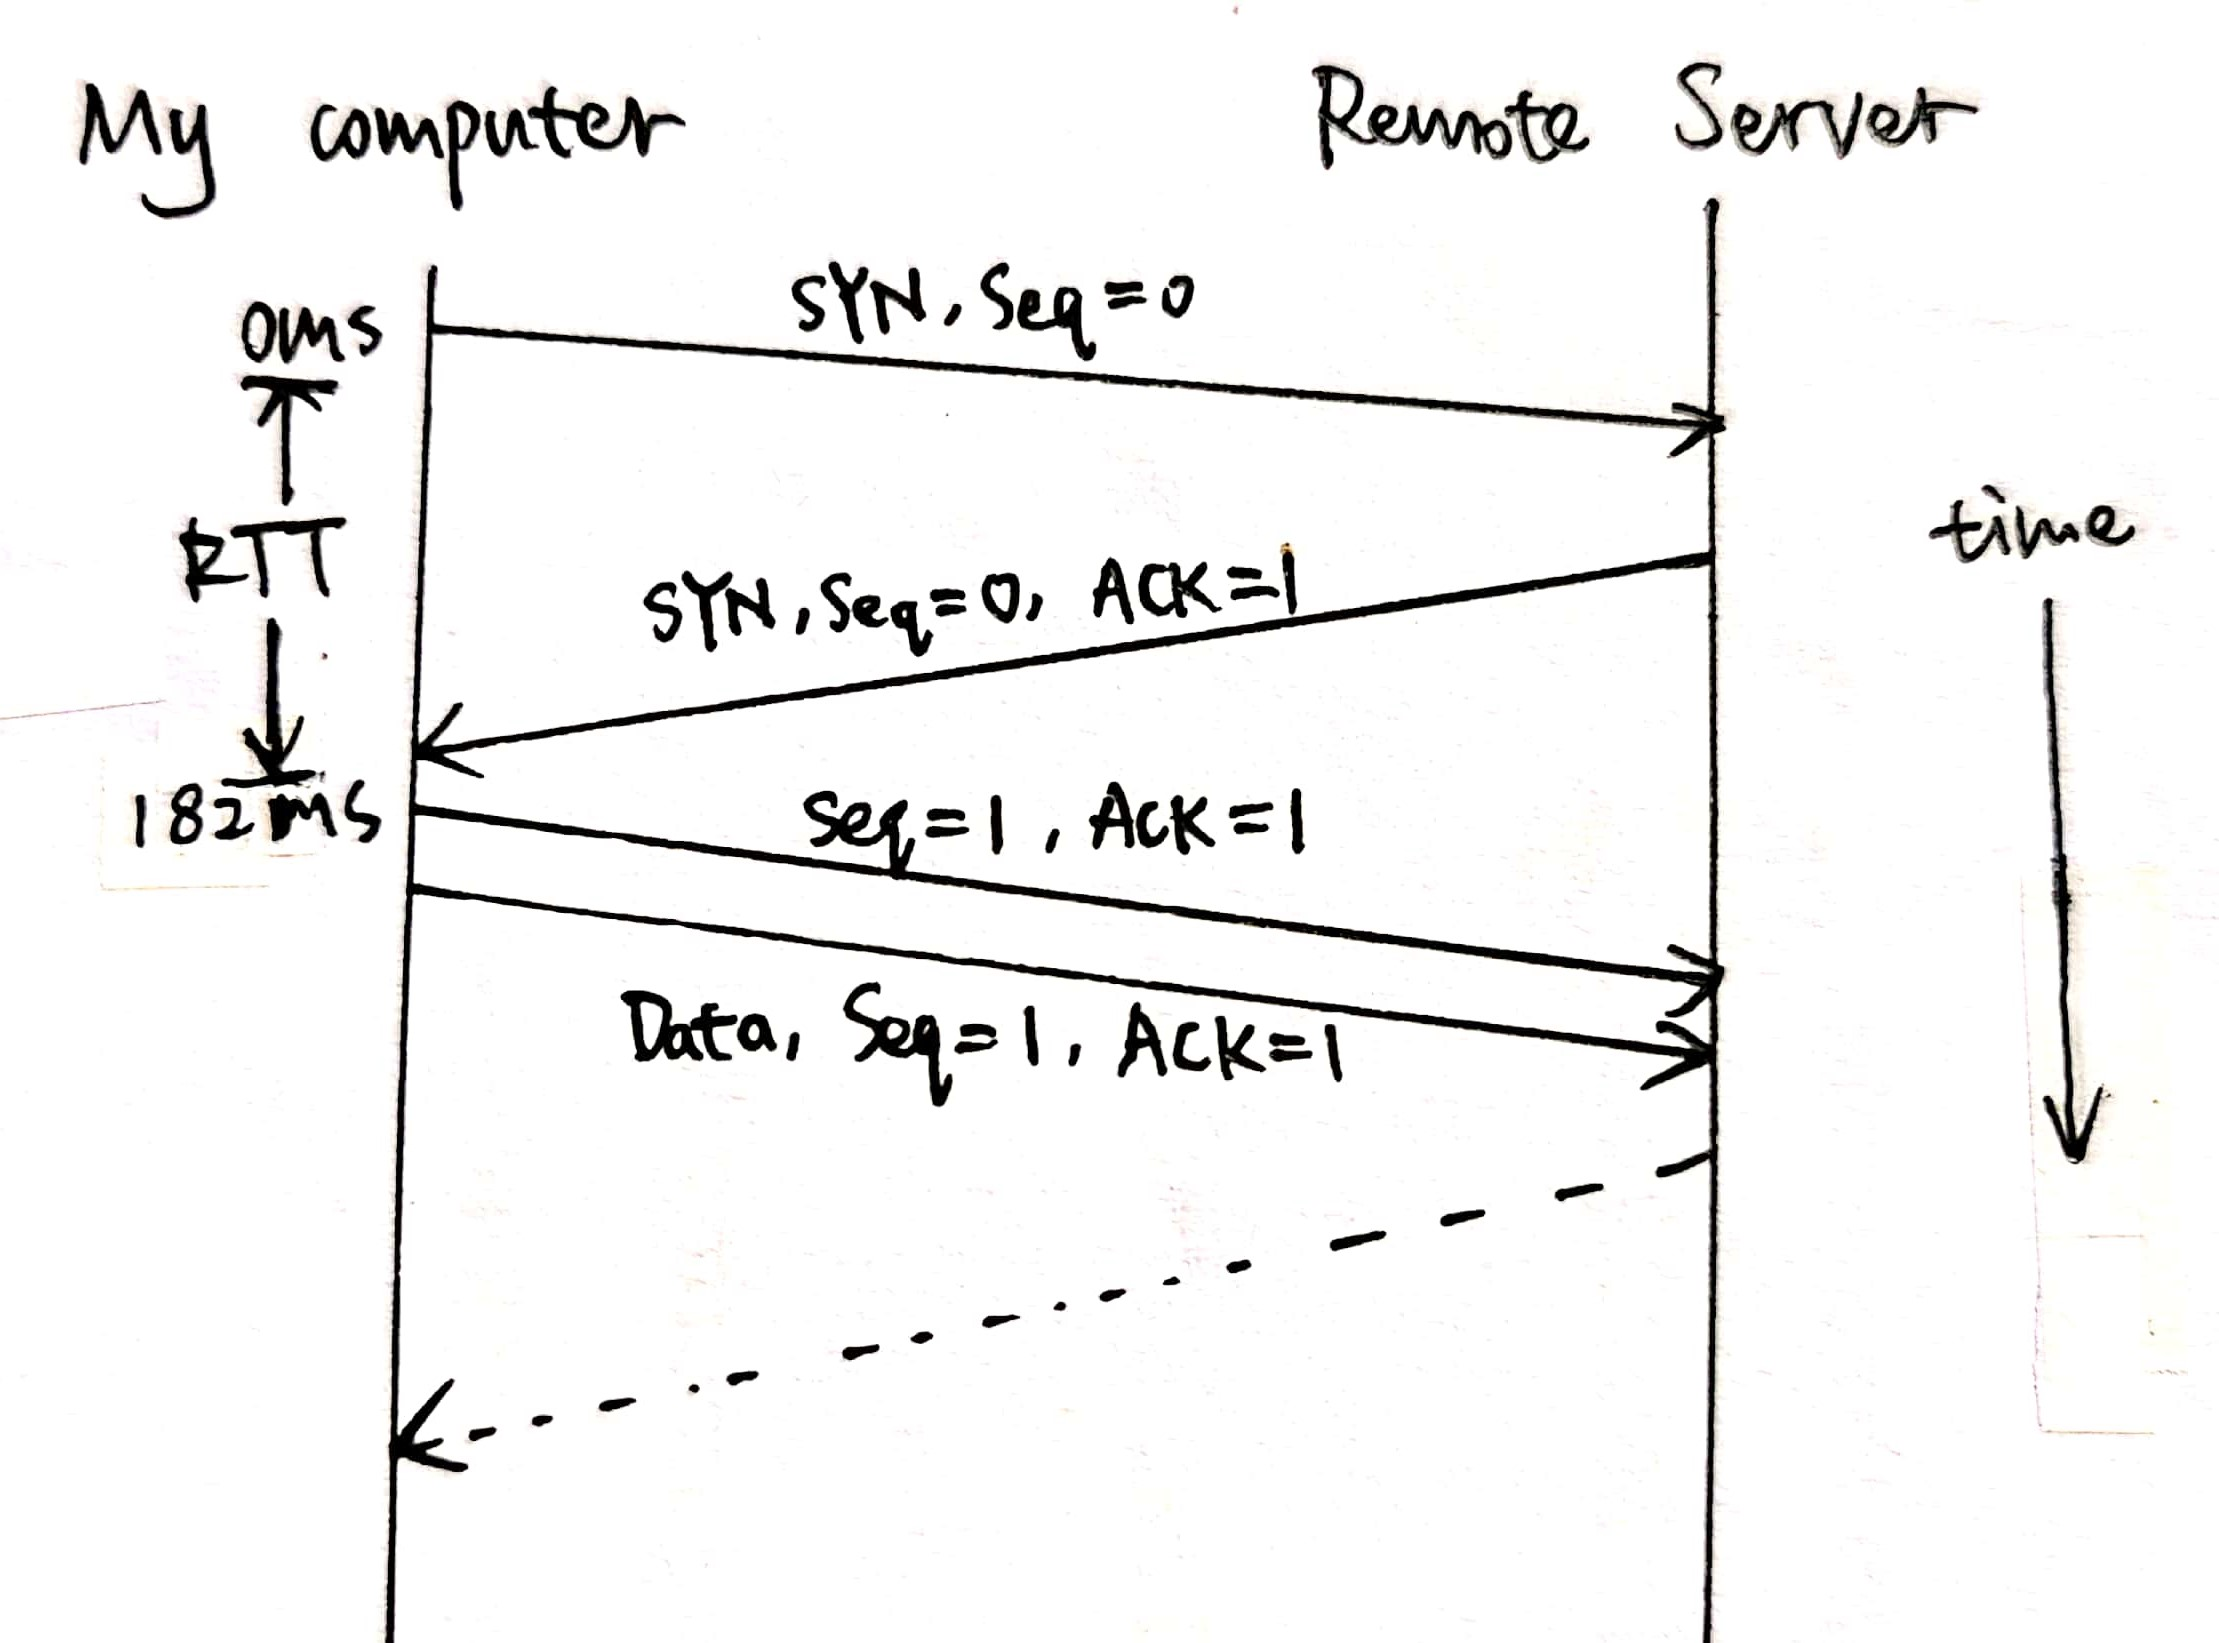
\includegraphics[scale=1]{2.jpg}
\caption{Screenshot of pinging 10 times from $h_3$ to $h_5$.}
\end{figure}
\item
\textbf{Path latency using ping.}
\par
The average round-trip time (RTT) between ($h_1$ and $h_5$) is $$\dfrac{142+143+143+145+144+144+143+146+144+144}{10}=143.8ms.$$ Link $L_1$, $L_2$ and $L_4$ are used and according to the given parameters, the theoretical delay between $h_1$ and $h_5$ is $(20+40+10)\times 2=140ms$. The round-trip time is close to this theoretical delay.
\begin{figure}[htbp]
\centering
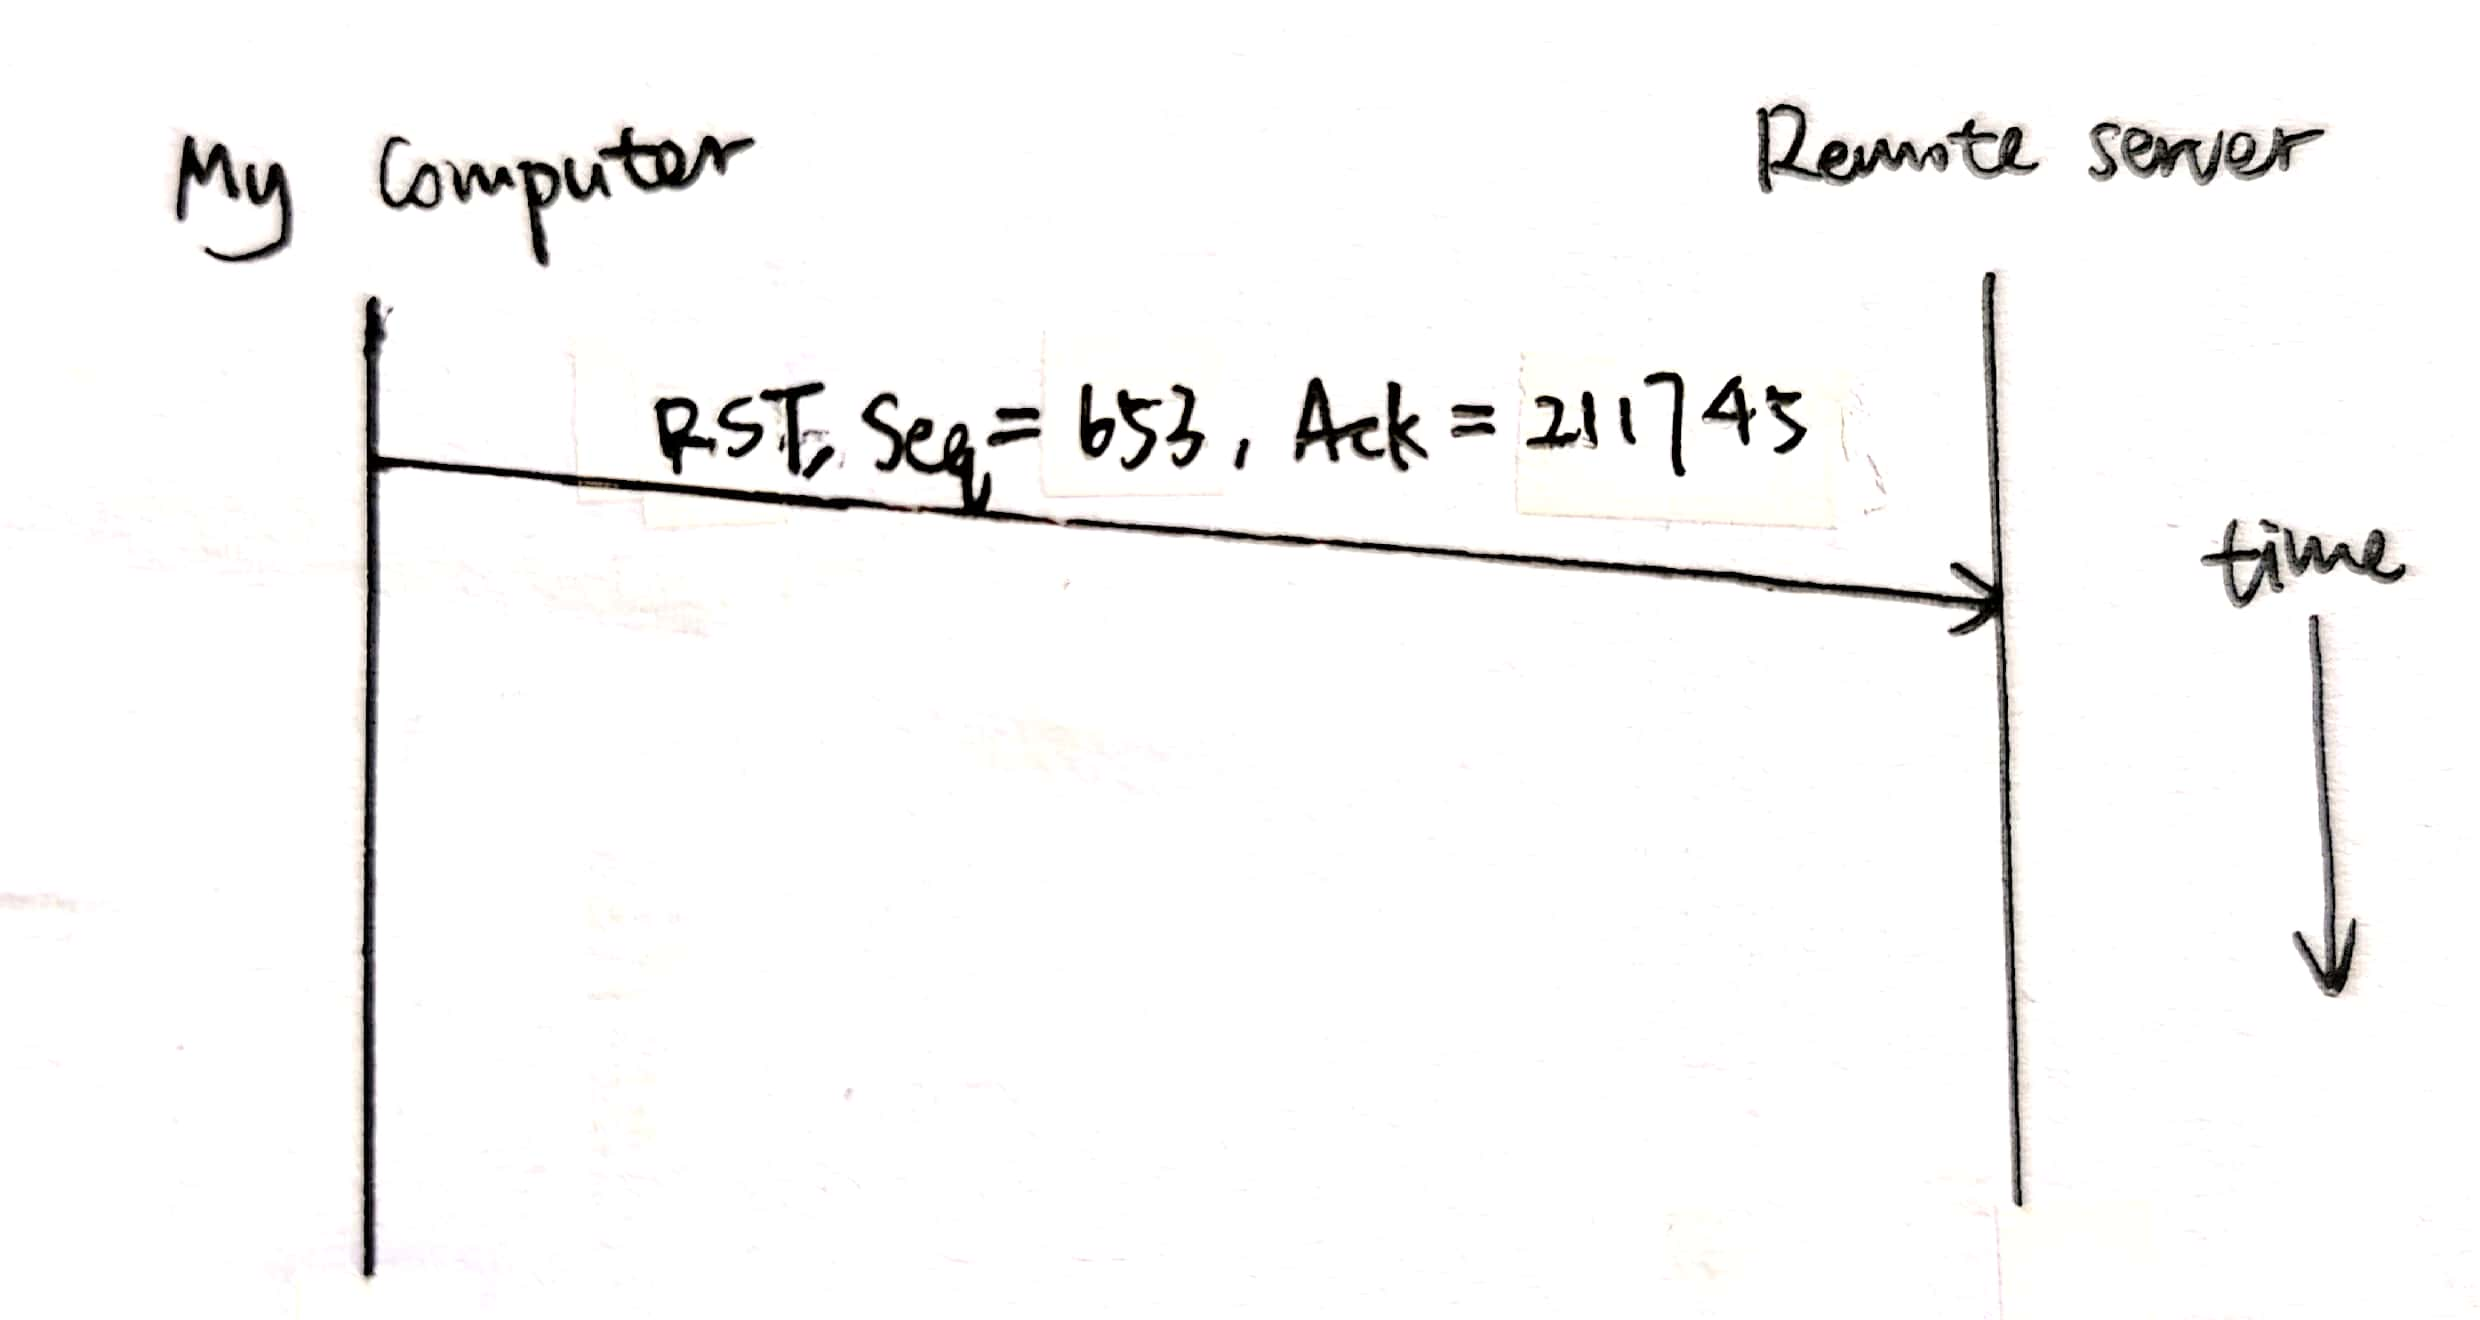
\includegraphics[scale=1]{3.jpg}
\caption{Screenshot of pinging 10 times from $h_1$ to $h_5$.}
\end{figure}
\par
The average round-trip time (RTT) between ($h_3$ and $h_4$) is $$\dfrac{142+141+143+146+144+143+142+142+143+143}{10}=142.9ms.$$ Link $L_2$ and $L_3$ are used and according to the given parameters, the theoretical delay between $h_3$ and $h_4$ is $(40+30)\times 2=140ms$. The round-trip time is close to this theoretical delay.
\begin{figure}[htbp]
\centering
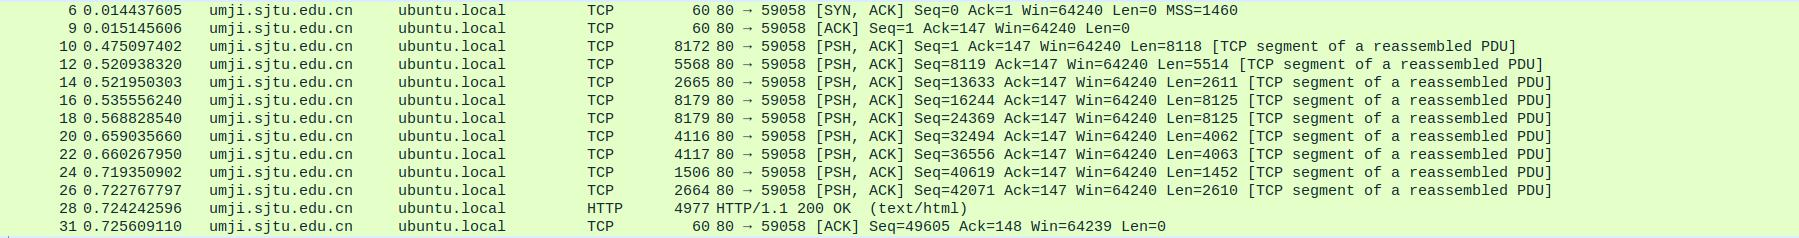
\includegraphics[scale=1]{4.jpg}
\caption{Screenshot of pinging 10 times from $h_3$ to $h_4$.}
\end{figure}

\item
\textbf{Link bandwidth using iperf.}
\par
The bandwidth result on the server $h_1$ is $40.8Mbps$. The bandwidth result on the client $h_2$ is $48.0Mbps$. They are both close to the link $L_1$'s bandwidth $50Mbps$. $59.2$ MBytes of data are transferred and received.
\begin{figure}[htbp]
\centering
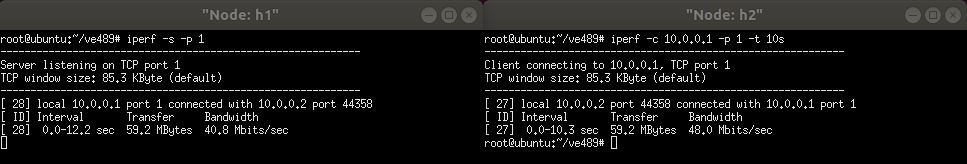
\includegraphics[scale=1]{5.jpg}
\caption{Screenshot of link bandwidth between $h_1$ and $h_2$.}
\end{figure}
\par
The bandwidth result on the server $h_3$ is $9.31Mbps$. The bandwidth result on the client $h_5$ is $11.1Mbps$. They are both close to the link $L_4$'s bandwidth $10Mbps$. $13.9$ MBytes of data are transferred and received.
\begin{figure}[htbp]
\centering
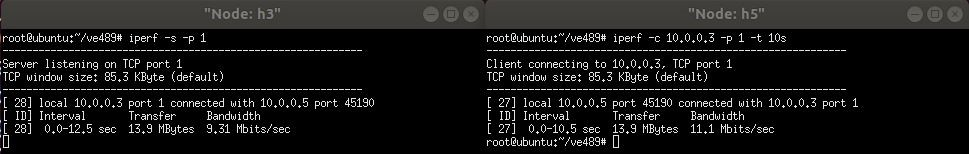
\includegraphics[scale=1]{6.jpg}
\caption{Screenshot of link bandwidth between $h_3$ and $h_5$.}
\end{figure}

\item
\textbf{Path throughput using iperf.}
\par
The bandwidth result on the server $h_1$ is $8.82Mbps$. The bandwidth result on the client $h_5$ is $11.3Mbps$. Link $L_4$ is the bottleneck link in this path and the result is close to $L_4$'s bandwidth $10Mbps$.
\begin{figure}[htbp]
\centering
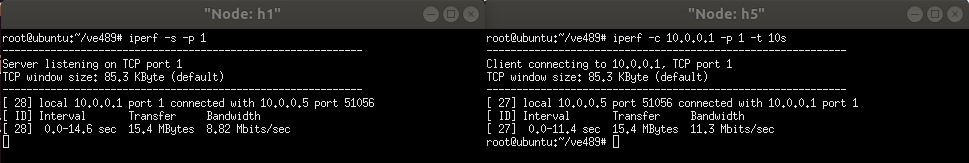
\includegraphics[scale=1]{7.jpg}
\caption{Screenshot of throughput between $h_1$ and $h_5$.}
\end{figure}
\par
The bandwidth result on the server $h_3$ is $17.6Mbps$. The bandwidth result on the client $h_4$ is $21.9Mbps$. Link $L_2$ is the bottleneck link in this path and the result is close to $L_2$'s bandwidth $20Mbps$.
\begin{figure}[htbp]
\centering
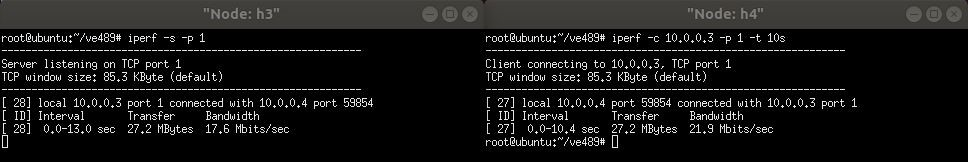
\includegraphics[scale=1]{8.jpg}
\caption{Screenshot of throughput between $h_3$ and $h_4$.}
\end{figure}

\item
\textbf{Multiplexing.}
\par
As shown in Figure 9, the latency and bandwidth is very similar to the previous results in question 2 and 4. Link $L_2$ is shared. And since the results doesn't change much from when they are transferring alone, they are sharing the link bandwidth fairly.
\begin{figure}[htbp]
\centering
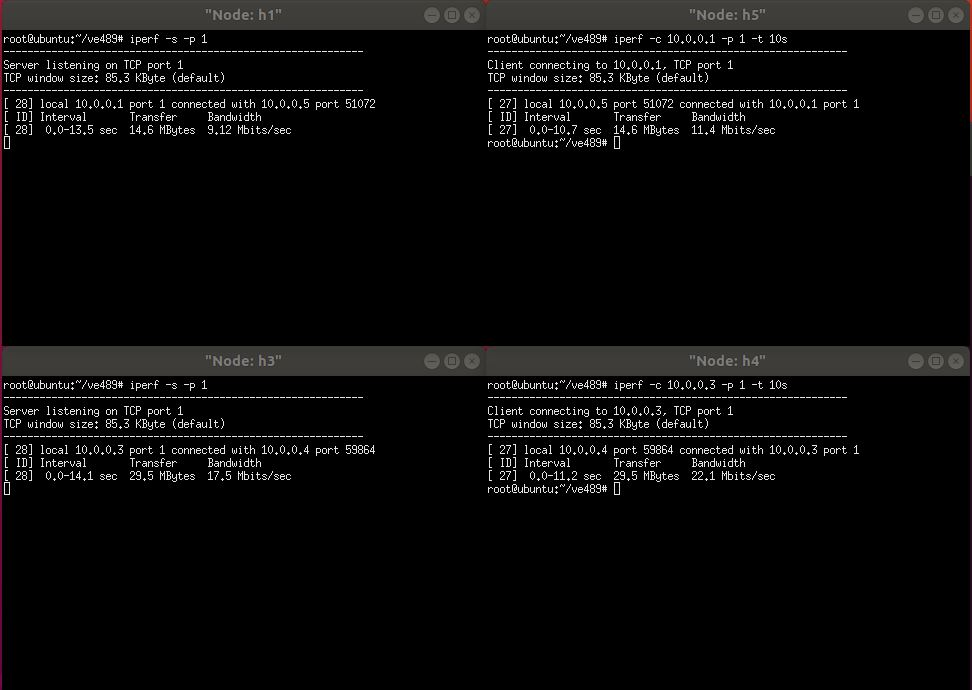
\includegraphics[scale=1]{9.jpg}
\caption{Screenshot of ($h_1$, $h_5$) and ($h_3$, $h_4$) sharing the same link.}
\end{figure}

\end{enumerate}
\section{Socket Programming}
\subsection{TCP File Transfer Server}
\noindent
\par
As shown in Figure 10, 11, 12, 13, these are the packets captured at the client. Client is at 10.0.0.2:8002 and server is at 10.0.0.1:8001.

\begin{figure}[htbp]
\centering
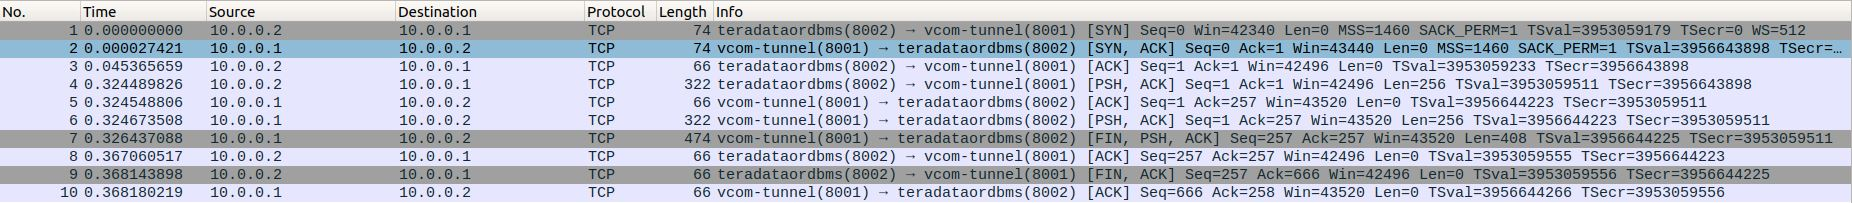
\includegraphics[scale=0.55]{12.jpg}
\caption{Screenshot of all packets captured by the clinet.}
\end{figure}

\begin{figure}[htbp]
\centering
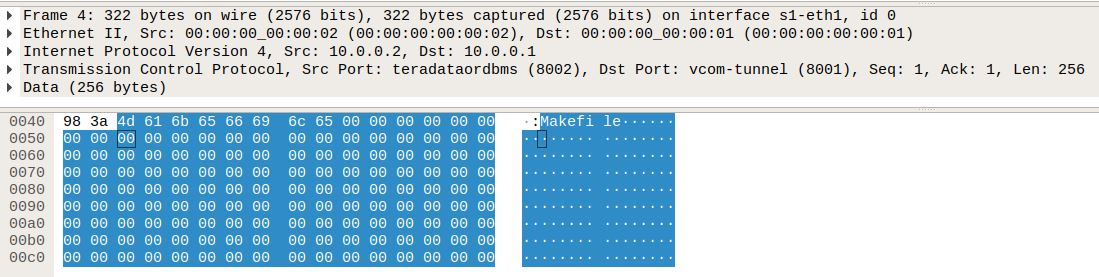
\includegraphics[scale=0.85]{13.jpg}
\caption{Screenshot of the packet that contains the requested filename.}
\end{figure}

\begin{figure}[htbp]
\centering
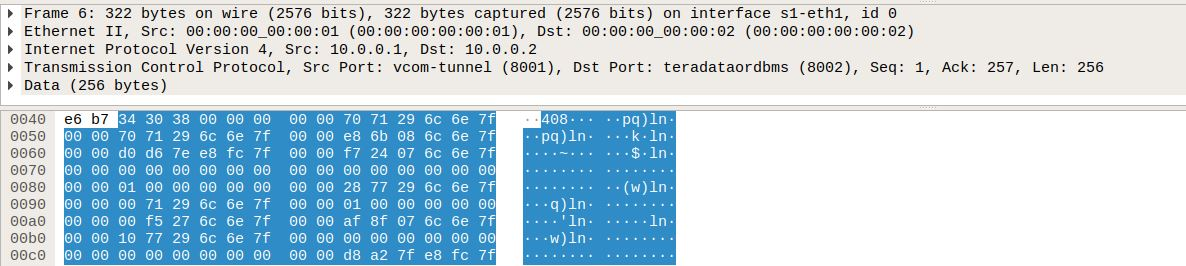
\includegraphics[scale=0.8]{14.jpg}
\caption{Screenshot of the packet that contains the file size.}
\end{figure}

\begin{figure}[htbp]
\centering
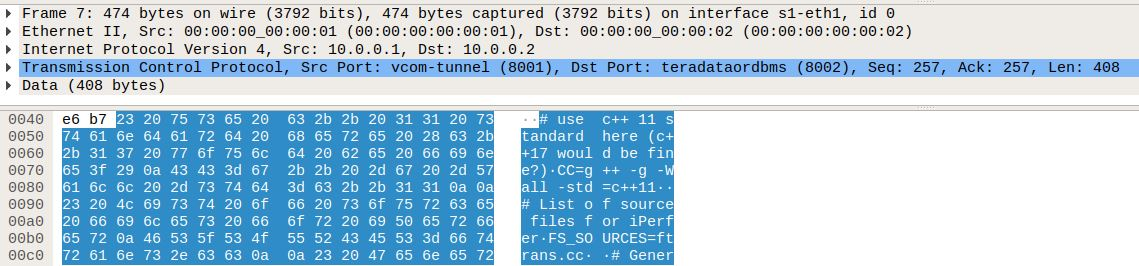
\includegraphics[scale=0.82]{15.jpg}
\caption{Screenshot of the packet that contains the file data, 408 bytes in total.}
\end{figure}
\section{Reliable Transmission}
\subsection{Implement a simple SR}
\begin{enumerate}[A]
\item No reordering, no loss, no error.\\

\fbox{%
  \parbox{0.95\textwidth}{%
$\#$ sender log\\
SYN 780 0 0 $\#$ initiate a connection\\
ACK 780 0 0 $\#$ receive ACK for the SYN (same seq as SYN)\\
DATA 0 1456 -1074344063 $\#$ send out 10 packets...\\
DATA 1 1456 -2050894268\\
DATA 2 1456 1460592462\\
DATA 3 1456 -879084444\\
DATA 4 1456 -838440118\\
DATA 5 1456 1573440664\\
DATA 6 1456 -822598369\\
DATA 7 1456 -1116097088\\
DATA 8 1456 279932998\\
DATA 9 1456 -868873766\\
ACK 1 0 0 $\#$ receive ACK for packet 1\\
DATA 10 1456 -1489524643 $\#$ window is slided, packet 10 is thus sent.\\
ACK 2 0 0 $\#$ receive ACK for packet 2\\
DATA 11 1456 443311922 $\#$ window is slided, packet 11 is thus sent.\\
...\\
FIN 780 0 0 $\#$ tear down the connection (same seq as SYN)\\
ACK 780 0 0 $\#$ receive ACK for the FIN\\
  }%
}

\fbox{%
  \parbox{0.95\textwidth}{%
$\#$ receiver log\\
SYN 780 0 0 $\#$ receive a connection request\\
ACK 780 0 0 $\#$ ACK with the same seq\\
DATA 0 1456 -1074344063 $\#$ receive packet 0\\
ACK 1 0 0 $\#$ ACK 1 (and slide window)\\
DATA 1 1456 -2050894268 $\#$ receive packet 1\\
ACK 2 0 0 $\#$ ACK 2 (and slide window)\\
...\\
FIN 780 0 0 $\#$ receive connection close request\\
ACK 780 0 0 $\#$ ACK the FIN\\
  }%
}


\item 10 percent loss, no reordering, no error.\\

\fbox{
  \parbox{0.95\textwidth}{
$\#$ sender log\\
..\\
DATA 19 1456 725513889\\
ACK 10 0 0\\
ACK 10 0 0 $\#$ still receive ACK 10\\
ACK 10 0 0\\
ACK 10 0 0\\
ACK 10 0 0\\
ACK 10 0 0\\
DATA 10 1456 -1489524643 $\#$ timeout is triggered, resend whole window\\
DATA 11 1456 443311922\\
DATA 12 1456 -267121725\\
DATA 13 1456 1330974691\\
DATA 14 1456 2109819272\\
DATA 15 1456 965284191\\
DATA 16 1456 -983191108\\
DATA 17 1456 1539359076\\
DATA 18 1456 -1934933216\\
DATA 19 1456 725513889\\
ACK 19 0 0\\
DATA 20 1456 -299260989 $\#$ receive ACK, proceed.\\
DATA 21 1456 -930311144\\
DATA 22 1456 943122041\\
DATA 23 1456 -1623696116\\
DATA 24 1456 -1706148246\\
...\\
  }%
}

\fbox{%
  \parbox{0.95\textwidth}{%
$\#$ receiver log\\
...\\
DATA 11 1456 443311922 $\#$ expect packet 10 but receive packet 11\\
ACK 10 0 0 $\#$ ACK 10\\
DATA 12 1456 -267121725 $\#$ expect packet 10 but receive packet 12\\
ACK 10 0 0 $\#$ ACK 10\\
DATA 13 1456 1330974691\\
ACK 10 0 0\\
DATA 14 1456 2109819272\\
ACK 10 0 0\\
DATA 15 1456 965284191\\
ACK 10 0 0\\
DATA 16 1456 -983191108\\
ACK 10 0 0\\
DATA 17 1456 1539359076\\
ACK 10 0 0\\
DATA 18 1456 -1934933216\\
ACK 10 0 0\\
DATA 10 1456 -1489524643 $\#$ finally receive packet 10\\
ACK 19 0 0 $\#$ ACK 19 now\\
DATA 12 1456 -267121725\\
ACK 19 0 0\\
DATA 13 1456 1330974691\\
ACK 19 0 0\\
...\\
  }%
}

\item 10 percent error, no reordering, no loss.\\

\fbox{
  \parbox{0.95\textwidth}{
$\#$ sender log\\
...\\
DATA 22 1456 943122041\\
ACK 14 0 0\\
DATA 23 1456 -1623696116\\
ACK 15 0 0\\
DATA 24 1456 -1706148246\\
ACK 15 0 0\\
ACK 15 0 0 $\#$ still receive ACK 15, packet 15 is probably corrupted\\
ACK 15 0 0\\
ACK 15 0 0\\
ACK 15 0 0\\
ACK 15 0 0\\
ACK 15 0 0\\
ACK 15 0 0\\
DATA 15 1456 965284191 $\#$ timeout is triggered, resend whole window, packet 15 is retransmitted\\
DATA 16 1456 -983191108\\
DATA 17 1456 1539359076\\
DATA 18 1456 -1934933216\\
DATA 19 1456 725513889\\
DATA 20 1456 -299260989\\
DATA 21 1456 -930311144\\
DATA 22 1456 943122041\\
DATA 23 1456 -1623696116\\
DATA 24 1456 -1706148246\\
ACK 17 0 0 $\#$ receive ACK, proceed\\
DATA 25 1456 -168693199\\
DATA 26 1456 1578006857\\
...\\
  }%
}

\fbox{%
  \parbox{0.95\textwidth}{%
$\#$ receiver log\\
...\\
DATA 14 1456 2109819272\\
ACK 15 0 0\\
DATA 15 1456 965284191 $\#$ 15 received but not ACKed because its payload is corrupted\\
DATA 16 1456 -983191108\\
ACK 15 0 0 $\#$ still ACK 15\\
DATA 17 1456 1539359076$\#$ 17 received but not ACKed because its payload is corrupted\\
DATA 18 1456 -1934933216\\
ACK 15 0 0\\
DATA 19 1456 725513889\\
ACK 15 0 0\\
DATA 20 1456 -299260989\\
ACK 15 0 0\\
DATA 21 1456 -930311144\\
ACK 15 0 0\\
DATA 22 1456 943122041\\
ACK 15 0 0\\
DATA 23 1456 -1623696116\\
ACK 15 0 0\\
DATA 24 1456 -1706148246\\
ACK 15 0 0\\
DATA 15 1456 965284191 $\#$ 15 is received correctly this time.\\
ACK 17 0 0 $\#$ ACK 17 now\\
...\\
  }%
}

\item Reordering, no error, no loss.\\

\fbox{
  \parbox{0.95\textwidth}{
$\#$ sender log\\
...\\
SYN 402536 0 0\\
ACK 402536 0 0\\
DATA 0 1456 -1074344063\\
DATA 1 1456 -2050894268\\
DATA 2 1456 1460592462\\
DATA 3 1456 -879084444\\
DATA 4 1456 -838440118\\
DATA 5 1456 1573440664\\
DATA 6 1456 -822598369\\
DATA 7 1456 -1116097088\\
DATA 8 1456 279932998\\
DATA 9 1456 -868873766\\
ACK 0 0 0\\
ACK 0 0 0 $\#$ still ACK 0\\
ACK 0 0 0\\
ACK 0 0 0\\
ACK 0 0 0\\
ACK 0 0 0\\
ACK 0 0 0\\
ACK 8 0 0 $\#$ finally ACK 8, meaning packet 0-7 are all received\\
DATA 10 1456 -1489524643\\
DATA 11 1456 443311922\\
DATA 12 1456 -267121725\\
DATA 13 1456 1330974691\\
DATA 14 1456 2109819272\\
DATA 15 1456 965284191\\
DATA 16 1456 -983191108\\
DATA 17 1456 1539359076\\
ACK 10 0 0 $\#$ ACK 10, meaning packet 0-9 are all received.\\
...\\
  }%
}

\fbox{%
  \parbox{0.95\textwidth}{%
$\#$ receiver log\\
...\\
SYN 402536 0 0\\
ACK 402536 0 0\\
DATA 2 1456 1460592462 $\#$ packets are reordered, 2 is received before 0\\
ACK 0 0 0 $\#$ ACK 0\\
DATA 3 1456 -879084444\\
ACK 0 0 0\\
DATA 7 1456 -1116097088\\
ACK 0 0 0\\
DATA 5 1456 1573440664\\
ACK 0 0 0\\
DATA 9 1456 -868873766\\
ACK 0 0 0\\
DATA 4 1456 -838440118\\
ACK 0 0 0\\
DATA 6 1456 -822598369\\
ACK 0 0 0\\
DATA 1 1456 -2050894268\\
ACK 0 0 0\\
DATA 0 1456 -1074344063 $\#$ packet 0 finally received\\
ACK 8 0 0 $\#$ ACK 8\\
DATA 8 1456 279932998\\
ACK 10 0 0\\
...\\
  }%
}

\item Reordering, 5 percent loss, 5 percent error.\\
\end{enumerate}
\subsection{Make sender more efficient - leverage duplicate ACK on sender side}

\begin{enumerate}[A]
\item 10% loss, no reordering, no error.\\

\fbox{
  \parbox{0.95\textwidth}{
$\#$ sender log\\
...\\
ACK 1 0 0\\
DATA 10 1456 -1489524643\\
ACK 2 0 0\\
DATA 11 1456 443311922\\
ACK 2 0 0\\
ACK 2 0 0 $\#$ receive three ACK 2\\
DATA 2 1456 1460592462 $\#$ resend packet 2\\
ACK 2 0 0\\
ACK 2 0 0\\
ACK 2 0 0 $\#$ receive three ACK 2\\
DATA 2 1456 1460592462 $\#$ resend packet 2\\
ACK 2 0 0\\
ACK 2 0 0\\
ACK 2 0 0 $\#$ receive three ACK 2\\
DATA 2 1456 1460592462 $\#$ resend packet 2\\
ACK 7 0 0 $\#$ finally ACK 7\\
DATA 12 1456 -267121725 $\#$ window is slided\\
...\\
  }%
}

\fbox{%
  \parbox{0.95\textwidth}{%
$\#$ receiver log\\
...\\
ACK 1 0 0\\
DATA 1 1456 -2050894268\\
ACK 2 0 0\\
DATA 3 1456 -879084444\\
ACK 2 0 0 $\#$ packet 2 is not received, still ACK 2\\
DATA 4 1456 -838440118\\
ACK 2 0 0\\
DATA 8 1456 279932998\\
ACK 2 0 0\\
DATA 9 1456 -868873766\\
ACK 2 0 0\\
DATA 6 1456 -822598369\\
ACK 2 0 0\\
DATA 5 1456 1573440664\\
ACK 2 0 0\\
DATA 10 1456 -1489524643\\
ACK 2 0 0\\
DATA 11 1456 443311922\\
ACK 2 0 0\\
DATA 2 1456 1460592462 $\#$ packet 2 is received\\
ACK 7 0 0 $\#$ ACK 7\\
...\\
  }%
}
\item Efficiency.\\
As shown in Figure 14 and 15, duplicate ACK makes the sender more efficient. When transmitting a 4.4MB file, the time the sender uses is almost halved after using duplicate ACK.
\begin{figure}[htbp]
\centering
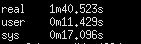
\includegraphics[scale=2]{16.jpg}
\caption{Screenshot of the time the sender use to send a 4.4MB file using simple SR.}
\end{figure}

\begin{figure}[htbp]
\centering
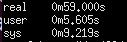
\includegraphics[scale=2]{17.jpg}
\caption{Screenshot of the time the sender use to send a 4.4MB file using duplicate ACK.}
\end{figure}
\item Make sure it transfers files reliably.\\
\end{enumerate}
\subsection{Make sender more efficient - send NACK on receiver side}
\begin{enumerate}[A]
\item 10% loss, no reordering, no error.\\

\fbox{
  \parbox{0.95\textwidth}{
$\#$ sender log\\
...\\
DATA 18 1456 -1934933216\\
ACK 10 0 0\\
DATA 19 1456 725513889\\
NACK 10 0 0 $\#$ receive NACK 10\\
DATA 10 1456 -1489524643 $\#$ resend packet 10\\
ACK 10 0 0\\
ACK 10 0 0\\
ACK 10 0 0\\
ACK 10 0 0\\
ACK 10 0 0\\
ACK 10 0 0\\
DATA 10 1456 -1489524643 $\#$ timeout is triggered, resend whole window\\
DATA 11 1456 443311922\\
DATA 12 1456 -267121725\\
DATA 13 1456 1330974691\\
DATA 14 1456 2109819272\\
DATA 15 1456 965284191\\
DATA 16 1456 -983191108\\
DATA 17 1456 1539359076\\
DATA 18 1456 -1934933216\\
DATA 19 1456 725513889\\
ACK 18 0 0 $\#$ receive ACK, proceed\\
DATA 20 1456 -299260989\\
DATA 21 1456 -930311144\\
...\\
  }%
}

\fbox{%
  \parbox{0.95\textwidth}{%
$\#$ receiver log\\
...\\
DATA 9 1456 -868873766\\
ACK 10 0 0\\
DATA 11 1456 443311922\\
NACK 10 0 0 $\#$ gap in window, NACK 10\\
DATA 12 1456 -267121725\\
ACK 10 0 0\\
DATA 13 1456 1330974691\\
ACK 10 0 0\\
DATA 14 1456 2109819272\\
ACK 10 0 0\\
DATA 15 1456 965284191\\
ACK 10 0 0\\
DATA 16 1456 -983191108\\
ACK 10 0 0\\
DATA 17 1456 1539359076\\
ACK 10 0 0\\
DATA 10 1456 -1489524643 $\#$ receive packet 10, proceed\\
ACK 18 0 0\\
...\\
  }%
}

\item Efficiency.\\
As shown in Figure 16 and 17, NACK makes the sender more efficient. When transmitting a 4.4MB file, the time the sender uses is almost halved after using NACK.
\begin{figure}[htbp]
\centering
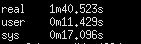
\includegraphics[scale=2]{16.jpg}
\caption{Screenshot of the time the sender use to send a 4.4MB file using simple SR.}
\end{figure}

\begin{figure}[htbp]
\centering
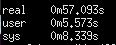
\includegraphics[scale=2]{18.jpg}
\caption{Screenshot of the time the sender use to send a 4.4MB file using NACK.}
\end{figure}

\item Make sure it transfers files reliably.\\

\end{enumerate}
\subsection{Throughput, delay and window size}
\noindent
\par
The file we transmit is a 4.4MB jpg file.\\
\\
When the delay is $0.01ms$ and the window size is 10, the real time is $15.870s$. The throughput is about $290721B/s$.\\
When the delay is $0.01ms$ and the window size is 5, the real time is $31.512s$. The throughput is about $146412B/s$.\\
When the delay is $10ms$ and the window size is 10, the real time is $22.310s$. The throughput is about $206801B/s$.\\
When the delay is $10ms$ and the window size is 5, the real time is $44.451s$. The throughput is about $103794B/s$.\\
When the delay is $50ms$ and the window size is 10, the real time is $46.407s$. The throughput is about $99419B/s$.\\
When the delay is $50ms$ and the window size is 5, the real time is $1m32.093s$. The throughput is about $50099B/s$.\\
When the delay is $100ms$ and the window size is 10, the real time is $1m16.549s$. The throughput is about $60272B/s$.\\
When the delay is $100ms$ and the window size is 5, the real time is $2m31.807s$. The throughput is about $30392B/s$.\\
\par
As we can see from the measurements and calculations, throughput increases as window size increases and it decreases as delay increases.
\begin{figure}[htbp]
\centering
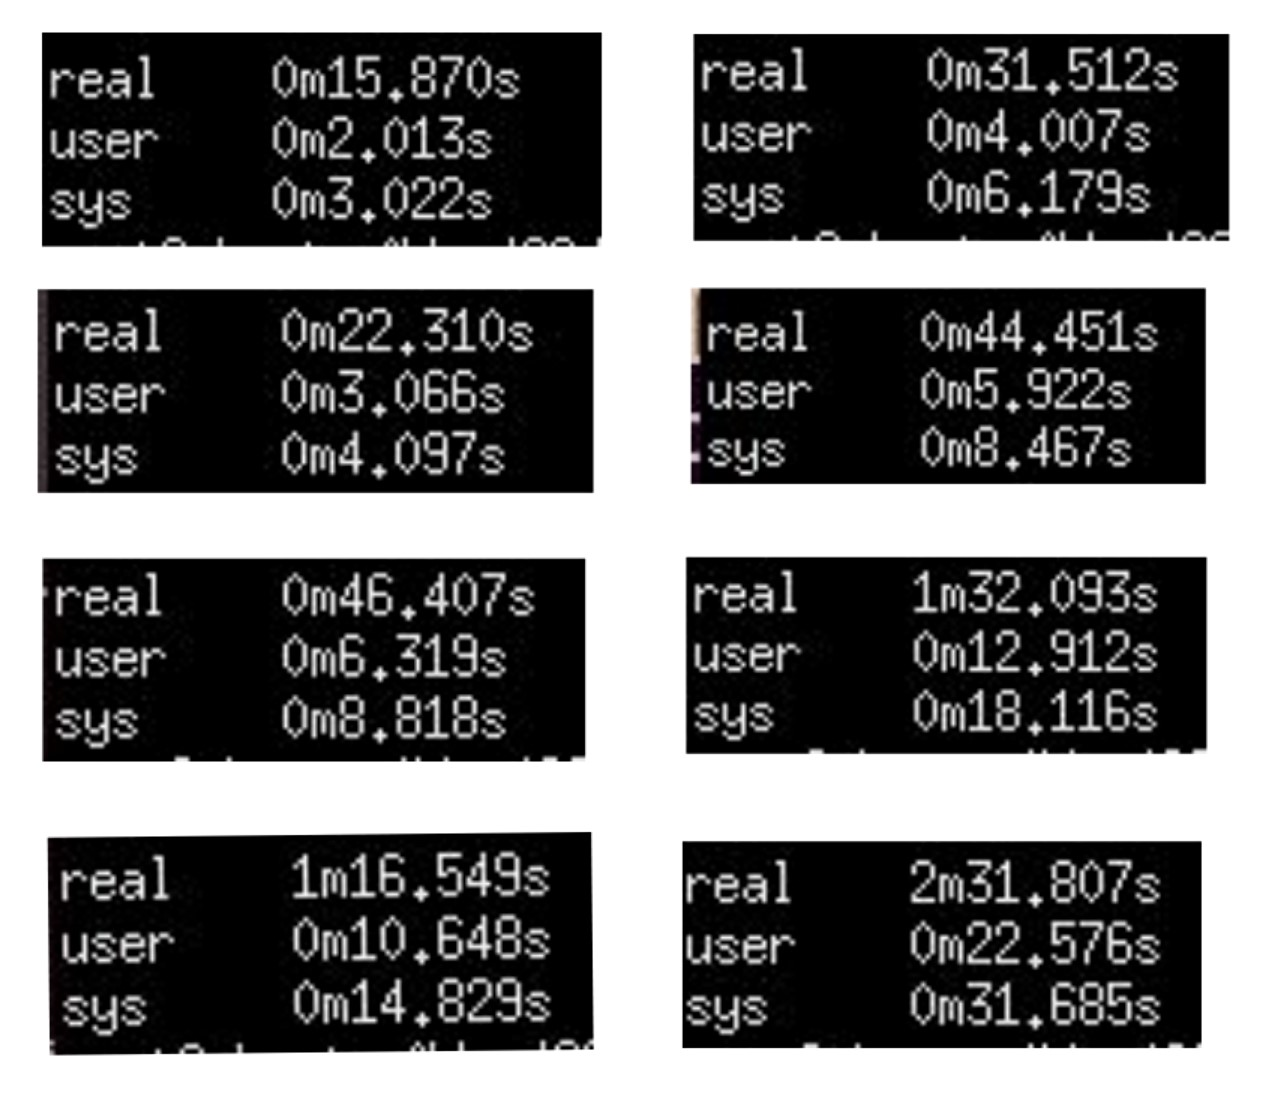
\includegraphics[scale=0.25]{23.jpg}
\caption{Screenshots of the time to transmit a 4.4MB file with different delays and window sizes.}
\end{figure}

\end{document}